% TODO eval all datasets for ldof ped mc, ldof pd sc
%TODO: explain statistical method: precission, recall, f1, density
%TODO: statistics: performance of selected set of methods applied on all datasets: HS_PD_SC, LDOF_PD_SC (classic), LDOF_PED_MC, LDOF_SD, LDOF_SED, SRSF_PED, SRSF_SED
%TODO: statistics: influence of lambda using LDOF_PD
%TODO: statistics: LDOF_PED_SC vs LDOF_PD_SC
%TODO: statistics: LDOF_PED_SC vs LDOF_PED_SC
%TODO: statistics: LDOF_PD_MC vs LDOF_SD
%TODO: statistics: LDOF_PED_MC vs LDOF_SED
%TODO: statistics: best case - tweak paras for a dataset.

%TODO: varying anzahl cluster: chair bonn/cerealbox 2:12, 3d lodf, unmerged results (ped sc, mc, mache plot anz.cluster/f1 score je methode plus prec-recall plot je methode
%TODO: mache overall performance stat. wenn standard params

\chapter{Results}
Finally, in this last section we describe how we evaluate our generated segmentations. Principally, the quality of a resulting segmentation is measured by comparing it against a manually drawn ground truth segmentation image. \\ \\
In the following the term $\textbf{P-affinity}$ refers to an affinity matrix generated by a product distance combination method. That means, that the affinity was produced by either $\textbf{PD}$ or $\textbf{PED}$. Please refer to the section $\ref{sec:affinity_matrix_impl}$ on page $\pageref{sec:affinity_matrix_impl}$ to re-read the definition of these modes. 

\section{Spectral Clustering Parameters}
\label{sec:spectral_clustering_parameters}
In this section we explain the default pipeline parameters which are used to generate the final results. Our motion segmentation pipeline exhibits many parameters since it consists of several stages such as the flow generation- affinity matrix computation- segmentation stage. Moreover, every stage implements different techniques to approach its specified tasks. Hence, a user has to specify both, which pipeline combination should be run and what parameter values of an specific method should be used. An example of all pipeline combinations is shown in figure $\ref{fig:pipeline_combinations}$. 
\begin{figure}[H]
\begin{center}
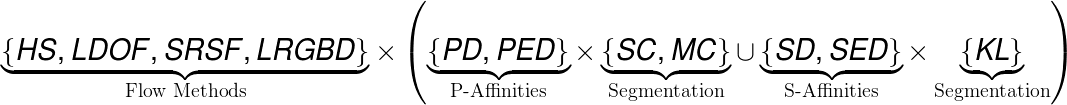
\includegraphics[width=1\linewidth] {evaluation/pipeline_combinations}
\end{center}
\caption[Pipeline Combinations]{A listing of all available pipeline combinations. Our pipeline implements a series of flow methods, various affinity computation modes and different segmentation techniques. Please notice that S-affinities can only be used in combination with the Kernighan-Lin Heuristic (KL). }
\label{fig:pipeline_combinations}
\end{figure}
In the following we give a brief description of several default assignments used in different pipeline stages. \\ \\
For generating the flow fields we rely on existing implementations offered by the authors. We do not attempt to modify any default settings of the utilized flow methods. For further information about those implementations, please refer to the author's papers or to section $\ref{sec:impl_optical_flow}$. \\ \\
The very first parameter we have to discuss is the sampling rate of the extracted traceable feature points, determined by a Harris-Corner detector, as discussed in section $\ref{sec:tracking_candidates}$. During our experiments we use every $8th$ pixel location. \\ \\
When computing a $\textit{P-affinity}$, either by running the mode \textit{PD} or $\textit{PED}$, we have to specify a certain value of $\lambda$. This parameter is used in equation $\ref{eq:prod_dist_affinity}$ to scale the similarity measure between two trajectories. We use$\footnote{We determined the defaults by trying out different values for $\lambda$ and took those which yielded the visually most promising results. Please note that this kind of parameter selection is by no means optimal.}$ $\lambda$ equals $0.1$ when running $PD$ and $\lambda = 10$ when running the affinity mode $PED$. The reason for using different $\lambda$ values is because PED and PD have different scales. \\ \\
In all of our motion segmentation methods, we set the cluster count they are supposed to solve for equals to two times the number of personally estimated moving objects. In other words the cluster count $CC$ is an estimate and defined as
\begin{equation}
	\text{CC} = 2 \times \text{Estimated Moving Objects in Dataset}
\label{eq:cc_def} 
\end{equation}
This estimation approach only takes into account very clearly, distinct moving objects and is thus probably underestimating the real moving object count. \\ \\
Segmentation methods that rely on P-affinities are utilizing a certain number of eigenvectors resulting from the eigenvalue decomposition of the Laplacian. For this eigenvector Count (EV) we use twice the number of the clusters the methods are supposed to solve for, i.e. this count is defined as
\begin{equation}
	\text{EV} = 2 \times \text{CC}
\end{equation}
Moreover, we set the relaxion parameter $\nu$ in our min-cut energy term defined in equation $\ref{eq:min_cut_energy_revisited}$ equals to the dimension of the affinity matrix times $10^-6$. \\ \\
In order to generate S-affinities we rely on the definition of equation $\ref{eq:sum_dist}$ to compute distances between trajectories. However, this equation is parameterized by several parameters $\beta$. We use the same $\beta$ values as defined in the paper $\cite{KB15b}$, which are equal to
\begin{equation}
\begin{aligned}
\bar{\beta}_0 = 6 \text{, } \beta_0 = 2 \text{, } \beta_1 = \beta_3 = -0.02 \text{ and } \beta_2 = -4
\end{aligned}
\end{equation}
The Kernighan-Lin partitioning method is always assigned with zero dummy vertices. \\ \\
Unless stated otherwise we rely on those parameter default parameter specifications to generate out results.

\section{Datasets}
\label{sec:datasets}
In this section we introduce the dataset we were using for generating our results. Our dataset are a diverse collection of videos, originating from various source. Some videos were captures by Microsoft's Kinect, some by Asus' Xtion. Some were manually captures and again others are from other authors. In particular the cars dataset is from the Middlebury dataset$\footnote{See \url{http://vision.middlebury.edu/stereo/data/}}$ and datasets prefixed by \textit{Bonn} are from Bonn's RGB-D Rigid Multi-Body Dataset $\footnote{See \url{http://www.ais.uni-bonn.de/download/rigidmultibody/}}$. \\ \\
We aim to work with a diverse collection of datasets. Meaning that we want to use datasets that capture different types of motions, are recorded in-and outdoor scenes and are captured by a static or moving cameras. Also, our implementation should be able to generated segmentations for long as well as for short sequences. \\ \\
Regularly, a dataset consists of the frames of a RGB-D video and the corresponding depth-and color camera calibrations. Moreover, for a selected set of frames we manually have drawn$\footnote{To draw these ground truth images using Gimp.}$ ground truth (\textbf{GT}) images. Please notice that all GT images were drawn according to the painter's opinion and thus do probably not truly correspond to the real ground truth. \\ \\
In the following a listing of our datasets, listing three of its frames, one of its ground truth motion segmentation images, a list of properties and a brief description what is happening in the video:
\begin{itemize}
\item \textbf{Cars}: \textbf{frames}: 19, \textbf{resolution}: $480 \times 640$, \textbf{depths}: No 
\begin{figure}[H]
\begin{center}
\subfigure[Frame 1]{
   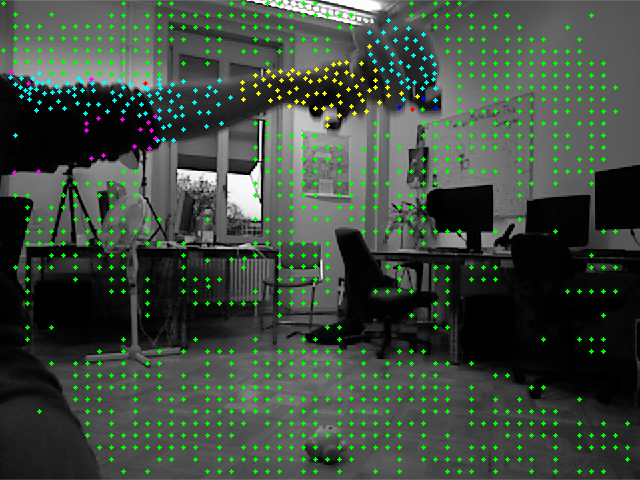
\includegraphics[width=0.22\linewidth] {evaluation/datasets/cars/1}
}
\subfigure[Frame 10]{
   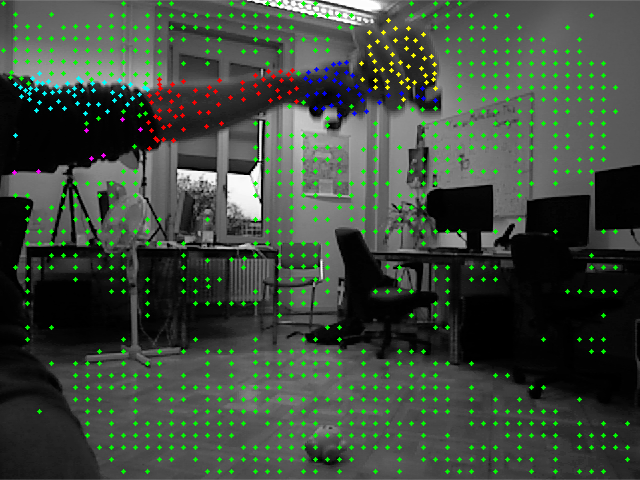
\includegraphics[width=0.22\linewidth] {evaluation/datasets/cars/10}
}
\subfigure[Frame 19]{
   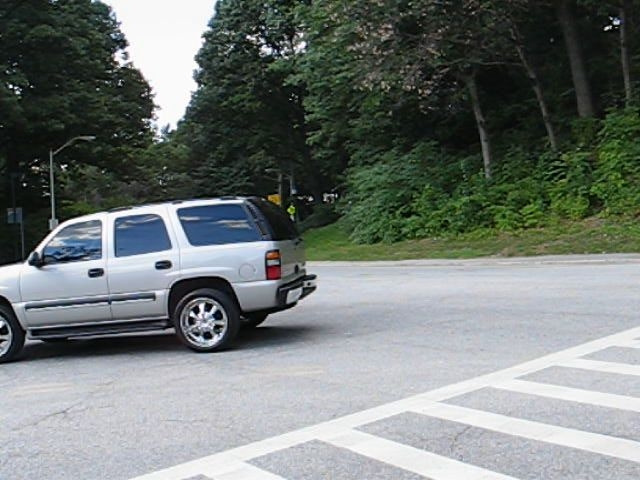
\includegraphics[width=0.22\linewidth] {evaluation/datasets/cars/19}
}
\subfigure[GT Frame 1]{
   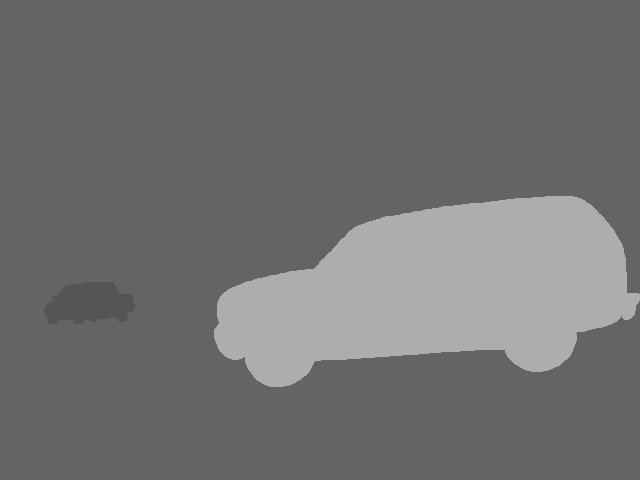
\includegraphics[width=0.22\linewidth] {evaluation/datasets/cars/gt1}
}
\end{center}
\caption[Dataset Bonn Cars]{An outdoor scene showing two cars, both moving to the left. One in the front and the other in the background. The camera is static.}
\label{fig:eval_datasets_cars}
\end{figure}
\item \textbf{Bonn Watercan}: \textbf{frames}: 58, \textbf{resolution}: $480 \times 640$, \textbf{depths}: Yes
\begin{figure}[H]
\begin{center}
\subfigure[Frame 4]{
   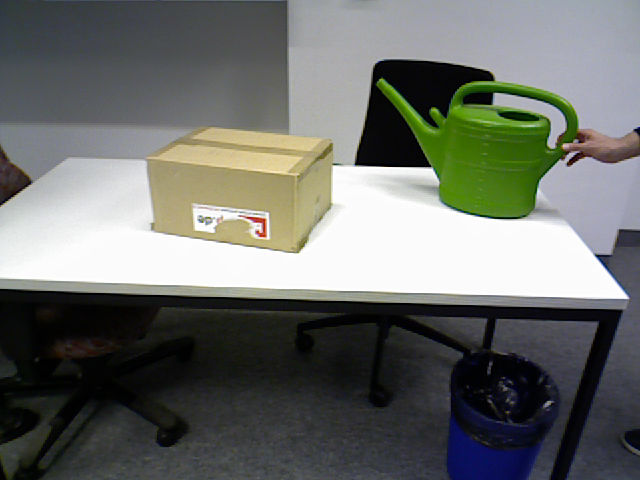
\includegraphics[width=0.22\linewidth] {evaluation/datasets/bonn_watercan/4}
}
\subfigure[Frame 31]{
   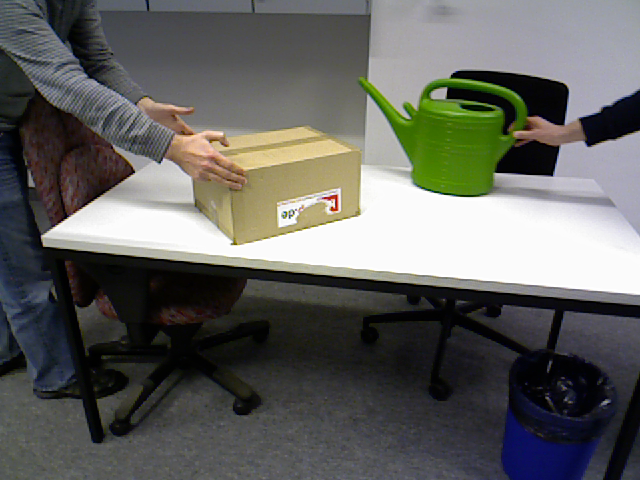
\includegraphics[width=0.22\linewidth] {evaluation/datasets/bonn_watercan/31}
}
\subfigure[Frame 58]{
   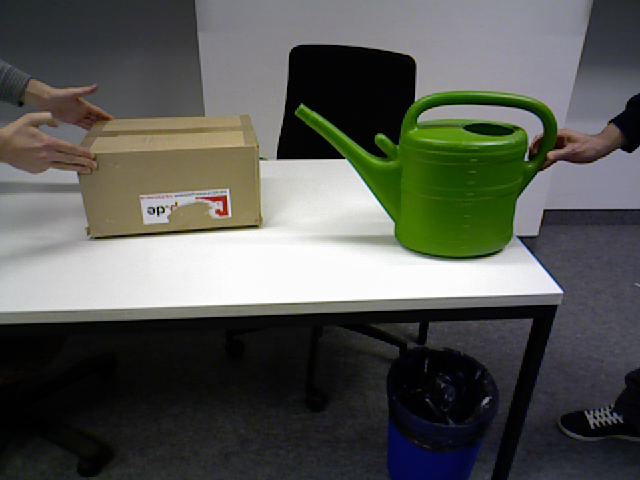
\includegraphics[width=0.22\linewidth] {evaluation/datasets/bonn_watercan/58}
}
\subfigure[GT Frame 4]{
   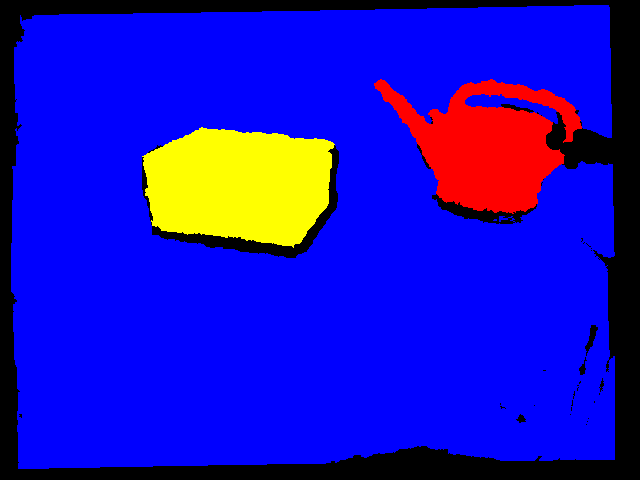
\includegraphics[width=0.22\linewidth] {evaluation/datasets/bonn_watercan/gt4}
}
\end{center}
\caption[Dataset Bonn Watercan]{An indoor scene showing two men psuhing different objects on a table. First, the man on the right side moves a water can along the table, then after a while the second man moves a packet from the left side of the table to its center. The camera is slightly shaking.}
\label{fig:eval_datasets_bonn_watercan}
\end{figure}
\item \textbf{Bonn Chairs}: \textbf{frames}: 58, \textbf{resolution}: $480 \times 640$, \textbf{depths}: Yes
\begin{figure}[H]
\begin{center}
\subfigure[Frame 15]{
   \includegraphics[width=0.22\linewidth] {evaluation/datasets/bonn_chairs/15}
}
\subfigure[Frame 30]{
   \includegraphics[width=0.22\linewidth] {evaluation/datasets/bonn_chairs/30}
}
\subfigure[Frame 45]{
   \includegraphics[width=0.22\linewidth] {evaluation/datasets/bonn_chairs/45}
}
\subfigure[GT Frame 15]{
   \includegraphics[width=0.22\linewidth] {evaluation/datasets/bonn_chairs/gt15}
}
\end{center}
\caption[Dataset Bonn Chairs]{An indoor scene showing a man moving a chair. First, he moved it to the left, then he rotates it slightly. The camera is slightly shaking.}
\label{fig:eval_datasets_bonn_chairs}
\end{figure}
\item \textbf{Bonn Cerealbox}: \textbf{frames}: 101, \textbf{resolution}: $480 \times 640$, \textbf{depths}: Yes
\begin{figure}[H]
\begin{center}
\subfigure[Frame 40]{
   \includegraphics[width=0.22\linewidth] {evaluation/datasets/bonn_cerealbox/40}
}
\subfigure[Frame 60]{
   \includegraphics[width=0.22\linewidth] {evaluation/datasets/bonn_cerealbox/60}
}
\subfigure[Frame 80]{
   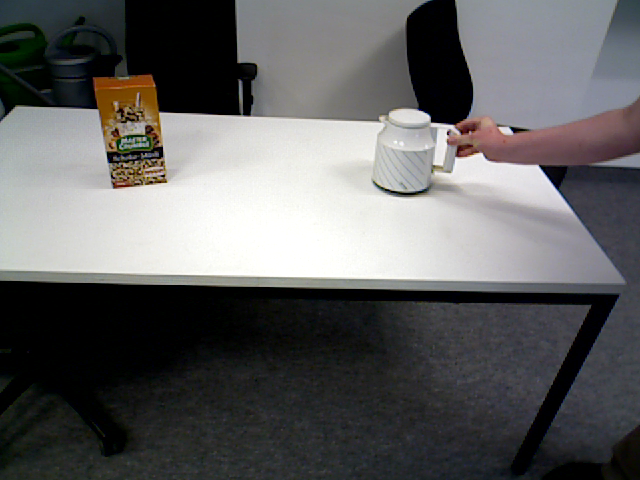
\includegraphics[width=0.22\linewidth] {evaluation/datasets/bonn_cerealbox/80}
}
\subfigure[GT Frame 40]{
   \includegraphics[width=0.22\linewidth] {evaluation/datasets/bonn_cerealbox/gt40}
}
\end{center}
\caption[Dataset Bonn Cerealbox]{An indoor scene showing a man moving a cup on table. The camera is slightly moving.}
\label{fig:eval_datasets_bonn_cerealbox}
\end{figure}
\item \textbf{Statue}: \textbf{frames}: 111, \textbf{resolution}: $480 \times 640$, \textbf{depths}: Yes
\begin{figure}[H]
\begin{center}
\subfigure[Frame 30]{
   \includegraphics[width=0.22\linewidth] {evaluation/datasets/statue/30}
}
\subfigure[Frame 60]{
   \includegraphics[width=0.22\linewidth] {evaluation/datasets/statue/60}
}
\subfigure[Frame 90]{
   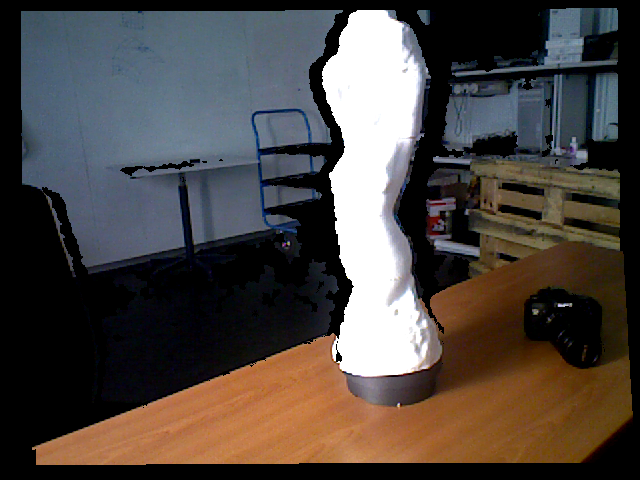
\includegraphics[width=0.22\linewidth] {evaluation/datasets/statue/90}
}
\subfigure[GT Frame 30]{
   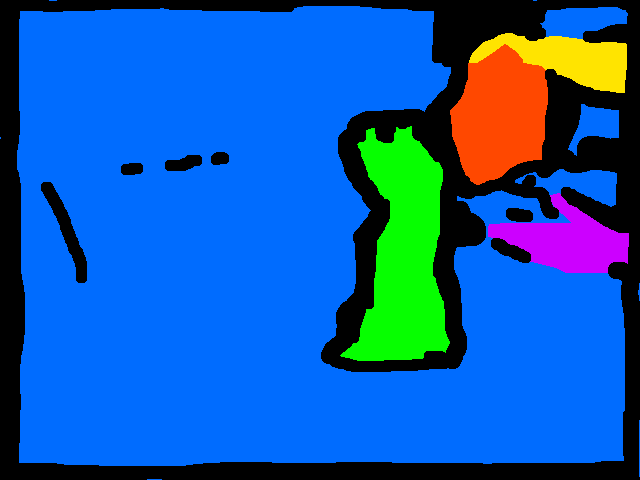
\includegraphics[width=0.22\linewidth] {evaluation/datasets/statue/gt30}
}
\end{center}
\caption[Dataset Statue]{An indoor scene a rotating statue. After a whole a man removes the upper part. We only see the man's hand. The camera is static.}
\label{fig:eval_datasets_statue}
\end{figure}
\item \textbf{Waving Arm}: \textbf{frames}: 104, \textbf{resolution}: $480 \times 640$, \textbf{depths}: Yes
\begin{figure}[H]
\begin{center}
\subfigure[Frame 20]{
   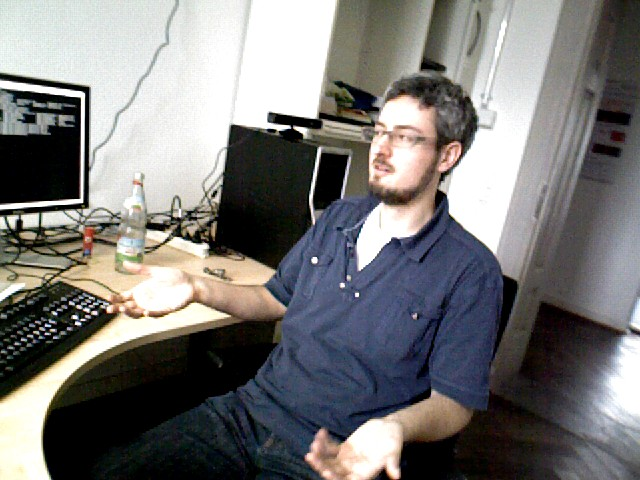
\includegraphics[width=0.22\linewidth] {evaluation/datasets/wh/20}
}
\subfigure[Frame 30]{
   \includegraphics[width=0.22\linewidth] {evaluation/datasets/wh/30}
}
\subfigure[Frame 40]{
   \includegraphics[width=0.22\linewidth] {evaluation/datasets/wh/40}
}
\subfigure[GT Frame 40]{
   \includegraphics[width=0.22\linewidth] {evaluation/datasets/wh/gt40}
}
\end{center}
\caption[Dataset Waving Hand]{An indoor scene showing a waving arm. The camera is static.}
\label{fig:eval_datasets_waving_hand}
\end{figure}
\item \textbf{Two Chairs}: \textbf{frames}: 61, \textbf{resolution}: $512 \times 424$, \textbf{depths}: Yes
\begin{figure}[H]
\begin{center}
\subfigure[Frame 15]{
   \includegraphics[width=0.22\linewidth] {evaluation/datasets/two_chairs/15}
}
\subfigure[Frame 40]{
   \includegraphics[width=0.22\linewidth] {evaluation/datasets/two_chairs/40}
}
\subfigure[Frame 60]{
   \includegraphics[width=0.22\linewidth] {evaluation/datasets/two_chairs/60}
}
\subfigure[GT Frame 15]{
   \includegraphics[width=0.22\linewidth] {evaluation/datasets/two_chairs/gt15}
}
\end{center}
\caption[Dataset Two Chairs]{An indoor scene showing two spinning chairs. The camera is static.}
\label{fig:eval_datasets_two_chairs}
\end{figure}
\item \textbf{One Chair}: \textbf{frames}: 101, \textbf{resolution}: $512 \times 424$, \textbf{depths}: Yes
\begin{figure}[H]
\begin{center}
\subfigure[Frame 45]{
   \includegraphics[width=0.22\linewidth] {evaluation/datasets/one_chair/45}
}
\subfigure[Frame 60]{
   \includegraphics[width=0.22\linewidth] {evaluation/datasets/one_chair/60}
}
\subfigure[Frame 75]{
   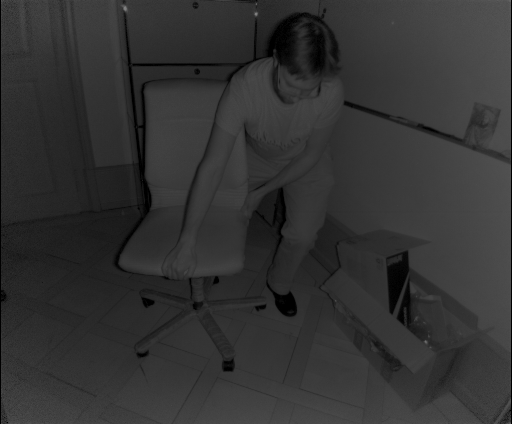
\includegraphics[width=0.22\linewidth] {evaluation/datasets/one_chair/75}
}
\subfigure[GT Frame 45]{
   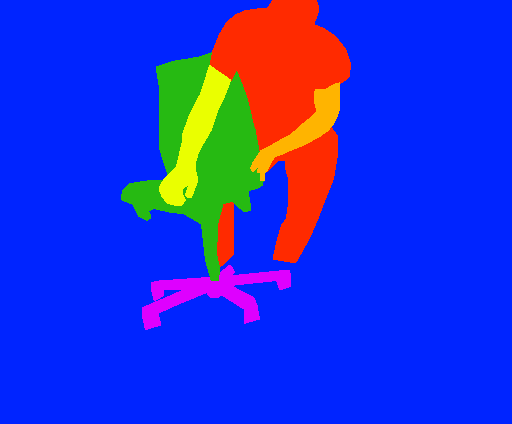
\includegraphics[width=0.22\linewidth] {evaluation/datasets/one_chair/gt45}
}
\end{center}
\caption[Dataset One Chair]{An indoor scene a man lifting a chair and spinning its lower part. The camera is static.}
\label{fig:eval_datasets_one_chair}
\end{figure}
\end{itemize}

\section{Segment Merger}
\label{sec:seg_merger}  
In this section we describe our technique to reduce oversegmentations produced by our pipeline. Our goal is to offer a mechanism that allows to evaluate the maximal potential of pipeline. However, some segmentation results are not clearly defined, such as fast movements resulting from non-rigidly moving objects. An good example of this problem case is when we attempt to segment a video showing a waving hand. That is rationale why we want to merge unclear segments. Moreover, we only allow to merger sparse segmentations, since our dense segmentation approach is basically blurring the sparse segments and thus is not yielding comparable results$\footnote{The more post-processing steps are added the more obfuscated the final segmentation quality gets.}$. This stage is invoked before running the evaluation program, implemented as a post-processing stage. \\ \\
Usually, the results generated by our pipeline exhibit an oversegmentation when comparing them against their ground truth. An example of such an oversegmentation is illustrated in figure $\ref{fig:merger_result_b}$. Ideally, before evaluating the quality, we would like to refine our over-segmented results in a way such that the total number of unnecessary or unclear segments is reduced. Therefore we want to merge  merge segments causing an oversegmentation. We achieve this by comparing the generated segments against a manually drawn ground truth image. For any generated segment we determine their best matching ground truth segment with respect to their overlapping parts. A conceptual visualization of our merging technique is visualized in figure $\ref{fig:merger_result}$. Please note that such a merging technique is just a hack. A more sophisticated method is described for merging clusters is presented in $\cite{OB14b}$.
\begin{figure}[H]
\begin{center}
\subfigure[Ground Truth Segmentation]{
   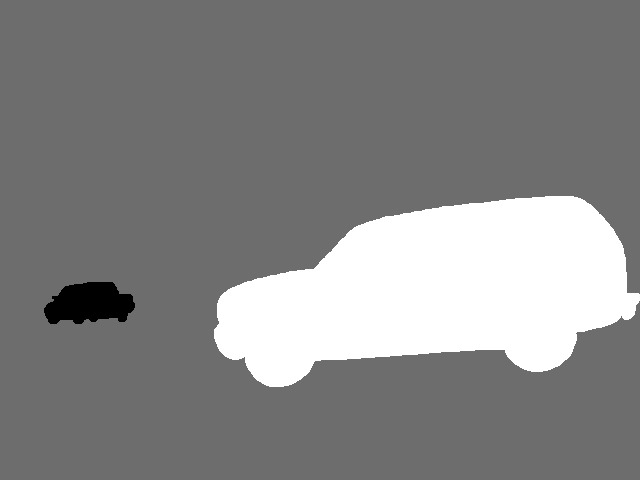
\includegraphics[width=0.47\linewidth] {implementation/merger/mask}
   \label{fig:merger_result_a}
}
\subfigure[Generated Segmentation]{
   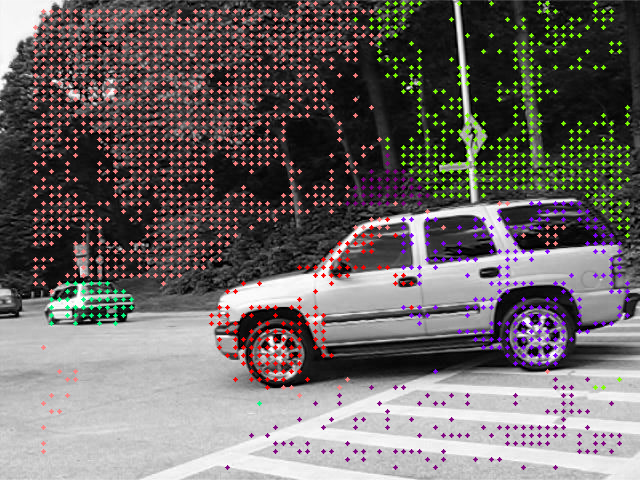
\includegraphics[width=0.47\linewidth] {implementation/merger/oversegmentation}
   \label{fig:merger_result_b}
}
~
\subfigure[Overlay Ground Truth / Segmentation]{
   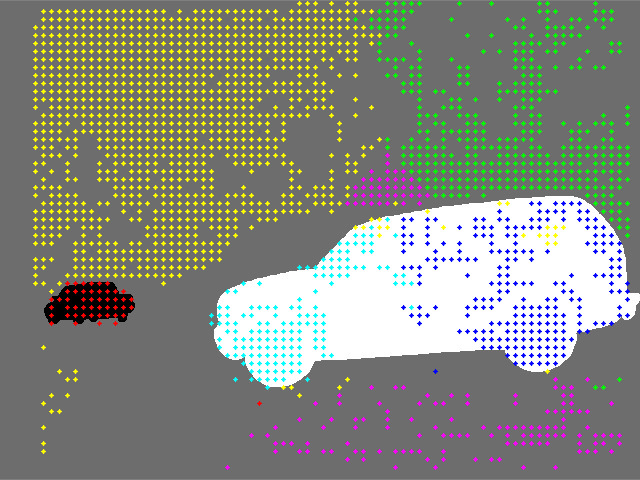
\includegraphics[width=0.47\linewidth] {implementation/merger/mask_segments_overlay}
   \label{fig:merger_result_c}
}
\subfigure[Merged Segmentation]{
   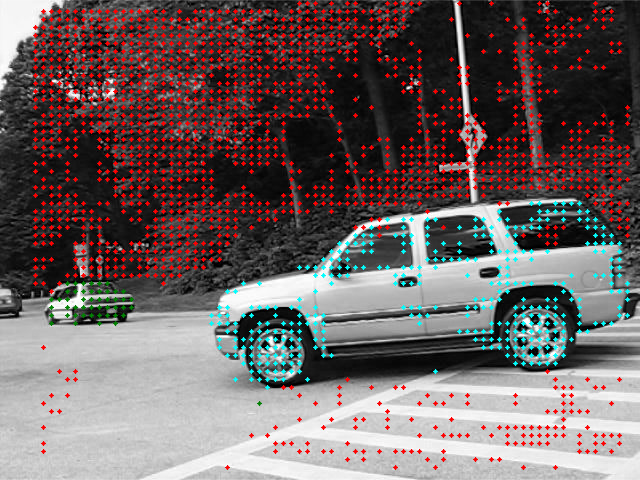
\includegraphics[width=0.47\linewidth] {implementation/merger/merged}
   \label{fig:merger_result_d}
}
\end{center}
\caption[Segmentation Merger]{Visualization of our segment merger's input and output. As an input it expects a ground truth segmentation (see figure $\ref{fig:merger_result_a}$) and a generated oversegmentation (see figure $\ref{fig:merger_result_b}$). As output it yields the merged segmentation as shown in subfigure $\ref{fig:merger_result_c}$.}
\label{fig:merger_result}
\end{figure}
A segmentation $S$ is basically a set of points in which every point is assigned to a certain segment identifier. In the following let us denote $S_j$ as the subset of points in $S$ that belong to the segmentation label $j$. Similarly, let $M$ denote the set of all ground truth points with their corresponding mask labels and $M_i$ the set of all points that belong to the ground truth mask $i$. To compute the merged segments we do the following: For every segment $S_j$ in $S$ we determine its best matching ground truth segment $M_i$ as defined in equation $\ref{eq:merging_label_formula}$. 
\begin{equation}
i = \argmaxl_{M_i \in M} \left\vert{S_j \cap M_i}\right\vert
\label{eq:merging_label_formula}
\end{equation}
The idea is to find the ground truth mask $i$ that yields the most point intersections with the currently considered segment $S_j$. Next, we update every point in $S_j$ by setting their segment label to $i$. After doing so we have computed the merged segmentation version of the initial oversegmentation. An example is shown in figure $\ref{fig:merger_result_c}$.

\section{Methodology}
\label{sec:methodology}
In this section we give a brief description about the methodology used to perform our experiments. \\ \\
We want to quantitatively evaluate the quality of segmentations produces by running different pipeline combinations. In particular we propose to evaluate the quality of how well moving objects were segmented. We use the datasets described in section $\ref{sec:datasets}$. Produced motion segmentations are compared against available ground truth images. While running the pipeline we rely on the defaults described in section $\ref{sec:spectral_clustering_parameters}$.\\ \\
Before evaluating the performance of generated segmentations, we run our segment merger, which is described in section $\ref{sec:seg_merger}$, as a post-processing step. The merged segments are quantitatively evaluated using different statistical measures. After running the merger, each GT object is assigned to at most one label. Therefore, the evaluation measures can be computed independently per object. In particular, for each segmentation result we compute their precession, recall and their f1 score by comparing them against their ground truth. The definition of these measures is listed in equation $\ref{eq:statistical_measures}$. 
\begin{equation}
\begin{aligned}
	& \text{precision} = \frac{\text{TP}}{\text{TP} + \text{FP}} \\
	& \text{recall} = \frac{\text{TP}}{\text{TP} + \text{FN}} \\
	& F_1 \text{ Score} = 2 \left( \frac{\text{precision} \times \text{recall}}{\text{precision} +\text{recall}} \right)
\end{aligned}
\label{eq:statistical_measures}
\end{equation}
The final reported outputs is the average value of these measured over all foreground objects. \\ \\
Finally some words about how we determined the quantities $TP$, $FP$ and $FN$. We only have to iterate over all points in every cluster and compare them against an available ground image. While doing so we count their true positives (\textbf{TP}), false negatives (\textbf{FP}) and their false negatives (\textbf{FN}). The exact definition of these quantities is listed in equation $\ref{eq:statistical_counts}$. For a given label $\alpha$ these measures are defined as:
\begin{equation}
\begin{aligned}
	\textbf{TP} &:= \text{Samples correctly labeled $\alpha$} \\
	\textbf{FP} &:= \text{Samples incorrectly labeled $\alpha$} \\
	\textbf{FN} &:= \text{Samples that were labeled $\alpha$ in GT but are attributed to a wrong label.}
\end{aligned}
\label{eq:statistical_counts}
\end{equation}
A detailed explanation of these measures can be found in the background section $\ref{sec:on_statistics_bg}$ on page $\pageref{sec:on_statistics_bg}$. \\ \\
One last note: During our evaluations we want to determine the quality of segmentations and the influence of design choices regardless of additional post-processing steps. Since our dense motion segmentation method basically performs a blurring on the sparse segmentation, and thus the quality is arbitrary influenced, we disallow using dense segmentations in our quantitative evaluation.

\section{Experiments}
\subsection{Parameter Experiments}
lediglich veranschauungszweck, untermalen, warum parameter so gewählt wie erklärt

ziel: alle varianten auf allen datasets
probleme: komplexity, dh alle kreuzkombinationen, so impractical that considering ldof and srsf

hs vergleichbar mit ldof und lrgbd 

zeige ldof sed kl
plots
u dessen plots (klein für var cluster)
% convergence i, ldof ped mc

\subsubsection{Convergence MC}
In the graph of figure $\ref{fig:two_chairs_ped_mc_iterations}$ we see a plot of the convergence rate of the MC segmentation method. The more iterations we run, the higher the F1-Score gets. However, we also observe, that the F1 Score is converging already after 3 iterations. This matches with our assumption that no more than 5 to 10 iterations have to be run when using the MC segmentation method.
\begin{figure}[H]
\begin{center}
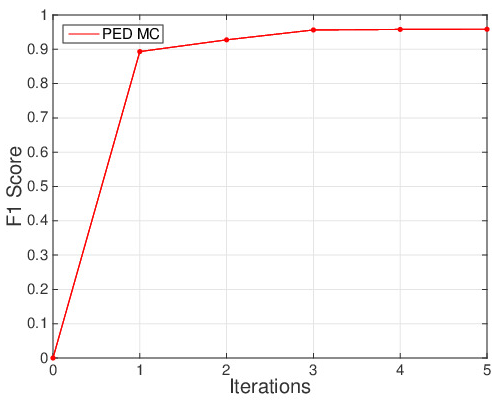
\includegraphics[width=0.47\linewidth] {evaluation/two_chairs/performance_iter/iter_f1}
\label{fig:two_chairs_ped_mc_iterations_b}
\end{center}
\caption[Convergence Rate MinCut Segmentation]{Visualizing the convergence rate of MC. We observe, that the more iterations are run, the higher the F1-Score gets. However}
\label{fig:two_chairs_ped_mc_iterations}
\end{figure}

\subsubsection{Choice for lambda}
\begin{table}[H]
\centering
\begin{tabular}{|c|c|c|c|c|}
\hline
\multicolumn{5}{|c|}{Performance Varying $\lambda$}                        \\ \hline
$\lambda$              & \textbf{Density} & \textbf{Precision} & \textbf{Recall} & \textbf{F1 Score} \\ \hline
5 & 0.59 & 99.70\%   & 57.99\%     & 73.33\%  \\ \hline
0.01 & 0.67 & 91.07\%   & 92.85\%     & 91.95\%  \\ \hline              
0.0001 & 0.67 & 47.91\%   & 49.62\%     & 48.75\%  \\ \hline
\end{tabular}
\caption[Cars Varying $\lambda$]{My caption}
\label{tab:cars_varying_lambas}
\end{table}

\subsubsection{Eigenvector Clustercount default}

\subsection{On exploring flow methods}
hs und lrgbd rausschmeisen

\subsection{Overall Performance}



\begin{table}[H]
\centering
\begin{tabular}{|c|c|c|c|}
\hline
\multicolumn{4}{|c|}{Using all datasets}                        \\ \hline
Method & \textbf{Precision} & \textbf{Recall} & \textbf{F1 Score} \\ \hline
LDOF PD SC & 63.52 \%   & 41.87\%     & 50.47\%  \\ \hline
LDOF PD MC & 58.69\%   & 57.86\%     & 58.27\%  \\ \hline
LDOF PED SC & 66.94\%   & 57.91\%     & 62.10\%  \\ \hline
LDOF PED MC & 64.11\%   & 67.27\%     & 65.65\%  \\ \hline                 
\end{tabular}
\caption[Overall Performance]{My caption}
\label{tab:overall_performance}
\end{table}


\begin{table}[H]
\centering
\begin{tabular}{|c|c|c|c|}
\hline
\multicolumn{4}{|c|}{Using compatible datasets}                        \\ \hline
Method & \textbf{Precision} & \textbf{Recall} & \textbf{F1 Score} \\ \hline
LDOF PD SC & 60.04 \%   & 35.99\%     & 45.00\%  \\ \hline
LDOF PD MC & 54.65\%   & 58.31\%     & 56.42\%  \\ \hline
LDOF PED SC & 63.85\%   & 59.68\%     & 61.69\%  \\ \hline
LDOF PED MC & 59.30\%   & 64.79\%     & 61.93\%  \\ \hline
SRSF PED MC & \textbf{76.52}\%   & \textbf{83.47}\%     & \textbf{79.84}\%  \\ \hline
SRSF PED SC & 60.23\%   & 49.62\%     & 54.41\%  \\ \hline 
SRSF PD MC & 61.85\%   & 55.06\%     & 58.25\%  \\ \hline
SRSF SED KL & 87.19\%   & 91.77\%     & 89.42\%  \\ \hline
Brox's GraphCut & 30.88\%   & 25.34\%     & 27.84\%  \\ \hline                   
\end{tabular}
\caption[Overall Performance]{My caption}
\label{tab:overall_performance}
\end{table}


\subsection{Properties}

\section{Runtime Measurements}
In this section we present actual runtime measurements resulting when running on the specified machine as defined in table $\ref{tab:used_hardware_specs}$. Please notice that by no means these measurements can be considered as statistical evident. The sole purpose of this section is to give the reader some further understanding about the pipeline and its usability in terms of \textit{how handy is this whole pipeline to use w.r.t. its runtime}. \\ \\
We start with measuring the runtimes of the utilized flow methods. For each method we run 3 dataset$\footnote{The dataset frames used to perform these measurement all exhibit a resolution 640 x 480 pixels.}$ and measured their total time to process their input. Each time measurement was divided by their total number of frames. The resulting timings were then finally averaged. Table $\ref{flow_method_runtimes}$ lists the average time in seconds that our flow methods require to process$\footnote{Here, the term process refers to generating the forward-and backward flow field of a frame.}$ one dataset frame. 
\begin{table}[H]
\centering
\begin{tabular}{|l|l|}
\hline
\textbf{Flow Method} & \textbf{Time per Frame} \\ \hline
HS & 18s \\ \hline
LDOF & 24s \\ \hline
SRSF & 72s \\ \hline
LRGBD & 674s \\ \hline
\end{tabular}
\caption[Flow Method Runtimes]{Listing of the average time of our flow methods required to process one dataset frame}
\label{flow_method_runtimes}
\end{table}
Next let us discuss the timings of the affinity matrix generation. Figure $\ref{fig:runtime_tra_track_affinity_gen}$ shows the timings in seconds of 261 measurements (blue dots) to accomplish the task of tracking a varying count of trajectories and generating their corresponding affinity matrix. Moreover, we fit a quadratic polynomial (red curve) on our measurements, since the runtime complexity of this pipeline stage is supposed to be in $\mathcal{O}(n^2)$ and $n$ denotes the trajectory count.
\begin{figure}[H]
\begin{center}
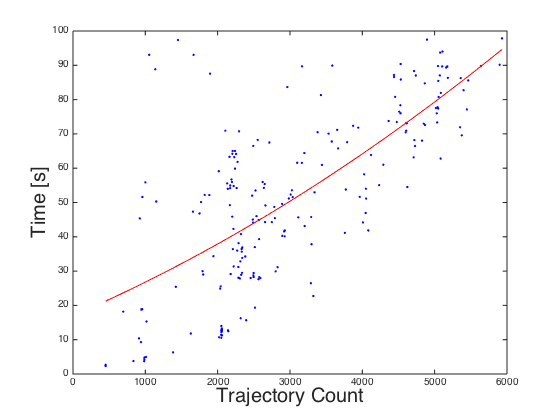
\includegraphics[width=0.8\linewidth] {evaluation/runtimes/affinity}
\end{center}
\caption[Runtime Trajectory Tracking and Generating Affinity Matrix]{Plotting the runtime (in seconds) of trajectory tracking and affinity matrix generation stage against the utilized trajectory count. The measurements are visualized as blue dots. A reconstructed quadratic curve is shown in red. The runtime of the evaluated stage is supposed to exhibit a quadratic complexity.}
\label{fig:runtime_tra_track_affinity_gen}
\end{figure}

%TODO: list runtime performance plots of our pipeline components
%TODO: list it in a table 


\section{Discussion}
After running our pipeline the following key observations can be stated:
\begin{itemize}
  \item Our pipeline can handle complex scenes: moving cameras, rotational movement.
  \item SRSF flows achieve the best segmentation results
  \item however, LDOF flows are still a solid choice and yield competitive results.
  \item when using P-affinities, then use Min-cut segmentation
  \item SED KL achieves the best results
  \item the best pipeline combination is SRSF SED KL 
  \item LRGBD flows are a very bad choice and yield poor motion segmentations
  \item using depth fields improves the quality of the segmentation results drastically
  \item when comparing our default pipeline setup against Brox' Min-Cut method, we obtain way better results.
  \item choosing the correct number of clusters and segments is a non-trivial task.
\end{itemize}











